%%% section
\section{Verification and Validation}
\label{sec: verification_and_validation} 

During the design and implementation stage, we had done many test case to ensure that the system should behave predictable manner. The test case can be categorize into 3 part:

\begin{enumerate}
    \item Truck Behaviour test.
    \item Communication behaviour test and
    \item Integration test
\end{enumerate}

This test lead us to improve the system design and implementation. For instance every component are design in the way that it can be executed independently from other component and can be tested individually. The test also give influence on our code pattern such as using switch case as listed in Listing \ref{code:code_satemachine} to realize state machine as in Figure \ref{img:controller_state_machine}.

%As we way this was implemented, different members of the team %implemented different things. Part of the last job to finish this %project was to merge all the module and finalize the testing. The %finalize version of the merge is represented by Figure \ref{img:}.

%%% IntegratedSystemUML
%\begin{figure}[ht]
%    \centering
%    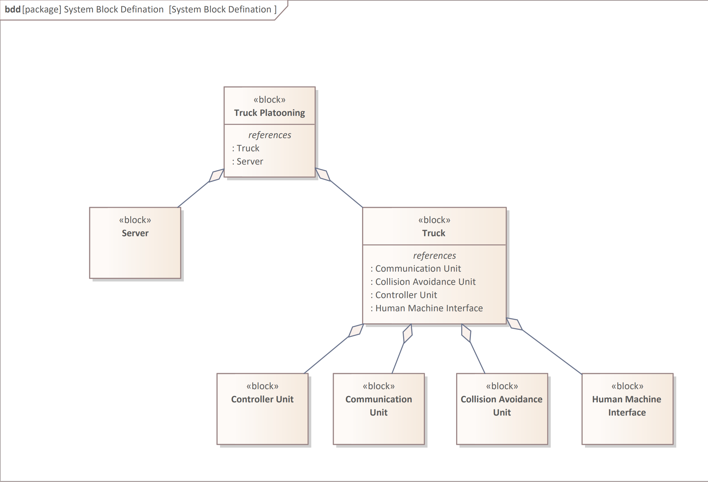
\includegraphics[width=0.5\textwidth]{images/IntegratedSystemUML.png}
%    \caption{IntegratedSystemUML}
%    \label{img:IntegratedSystemUML}
%\end{figure}


%%% subsection
\subsection{Truck behaviour test}
\label{subsec:truck_behaviour_test } 

As we explained before, the truck consist of 3 component which is controller, communication module and driver interface. Since the communication module is apart of communication, those components are tested together with the serve in communication test part.

the controller are tested to ensure that the sequence of state are predictable based on given event and input. For instance, when a leader is found (by adding a dummy truck id and information), the controller shall change from waiting state to follower state.

for the driver interface component, test were conducted in order to ensure that the component doesn't effect the behaviour of other component such as preventing other component from being executed and also to ensure correct output when an input is given from the user. This is partially explained in section \ref{subsec:driver_interface}.
The integration test (driver interface and controller) implemented for the truck was to ensure the behaviour of the controller output  were working as planned. 

%In such case that the truck will do the corresponding initialization %sequences and then select a role depending on the information available %on  the server.
%The following step was to make sure that the truck object will execute %in a ‘n’ amount of time as expected when an input was provided as a %user. 



%All this cases with the truck set as a leader, as for this test
%The validation of the state machine was a little complicated as most of the events needed to be simulated as we did not had the system as a whole in this point. However, for this validation a simple statement of prints was sufficient to test that depending on the event, the system%would change its state, such as in Listing \ref{code:code_satemachine}.



%%% code state machine event based
\begin{lstlisting}[language=c++, caption=Main process of a controller. Realization of controller state machine , label=code:code_satemachine]

while(true){
    next_state_computer(self_truck->event_handler); //set next state
    self_truck->event_handler = ev_any; // reset event handler
    switch(next_state){
        case initial:
            self_truck->event_handler = state_initial();
            break;
        case waiting:
            self_truck->event_handler = state_waiting();
            break;
        case leader:
            self_truck->event_handler = state_leader();
            break;
        case follower:
            self_truck->event_handler = state_follower();
            break;
        case system_stop:
            self_truck->event_handler = state_system_stop();
            break;
        default:
            break;
    }
}
\end{lstlisting}


%%% subsection
\subsection{Communication behaviour test}
\label{subsec:communication_behaviour_test} 

Client connect to server
Server accepting multiple client
Server forwarding message


%%% subsection
\subsection{Integration test}
\label{subsec:integration_test}

Now we are at the final stage of testing, the full integration test. For this case we already consider to have a compliable code of the whole system as shown in Figure \ref{img:system_bdd}. 
For this case we already tested the Server-Client scenario, where we have one server and multiple clients, as well as the system for the truck, so lastly we need to test the system as a whole. In this test scenario we do the following procedure:

\begin{enumerate}
\item 	Run Server.exe - to initialize the server which we are using to communicate.
\item	Run Truck.exe - to initialize a first truck and we set with ID = 1. 
\item	Run as many trucks as our machine can handle, as these are the follower's trucks, but the ID cannot be repeated. When all the trucks are connected to the server you should be able to see information such as in Figure \ref{img:SystemTest_Init}. This will mean that all the trucks are connected to the server and receiving information from the leader.
\end{enumerate}

The next step for the integration test was to start moving the leader truck and wait to see if all the information was being received by the followers. In this case the integration was a success since, in the integration test we got a positive response from all the followers, shown in Figure \ref{img:SystemTest_Listen}.

From the Figure \ref{img:SystemTest_Listen}, we see from the server side (bottom left) that all the trucks are synchronized to the leader. Since the logical clock in this implementation is done in a way that we only increase on every event that sets a new speed or direction. 

For finish this system test, a last thing was needed and that was to kill the process of the leader truck, so a new truck could assume its role. As we can see in Figure \ref{img:SystemTest_Case}, we kill the first 2 trucks simulating that they left the platoon and now the next truck in the platoon can assume the leadership, which in this case is the truck with an ID = 3.

%%% IntegratedSystemUML
%\begin{figure}[ht]
%    \centering
%    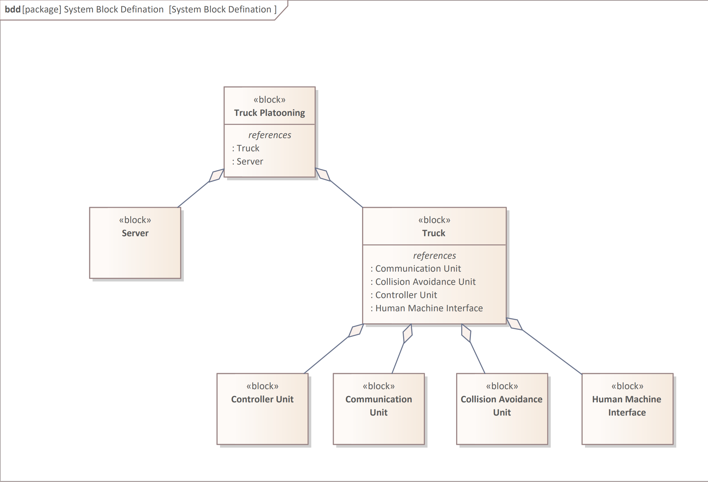
\includegraphics[width=0.5\textwidth]{images/IntegratedSystemUML.png}
%    \caption{IntegratedSystemUML}
%    \label{img:IntegratedSystemUML}
%\end{figure}

%%% SystemTest_Init
\begin{figure}[ht]
    \centering
    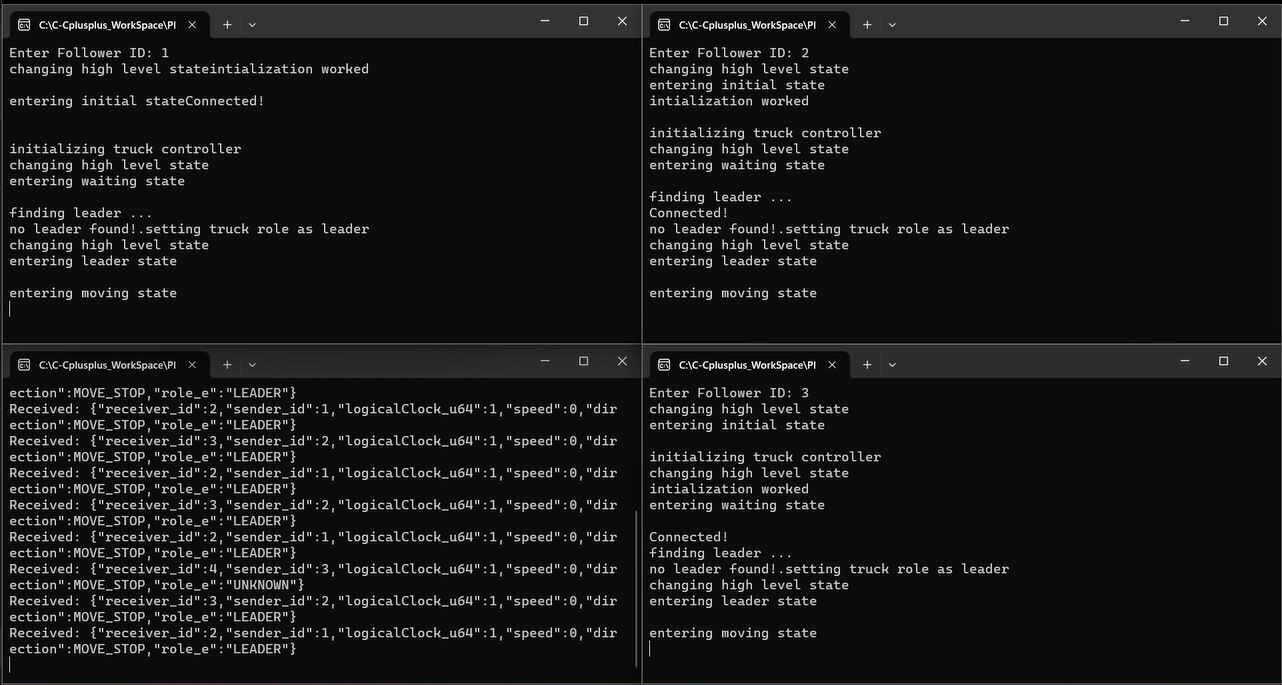
\includegraphics[width=0.5\textwidth]{images/SystemTest_Init.png}
    \caption{System initialization test}
    \label{img:SystemTest_Init}
\end{figure}

%%% SystemTest_Listen
\begin{figure}[ht]
    \centering
    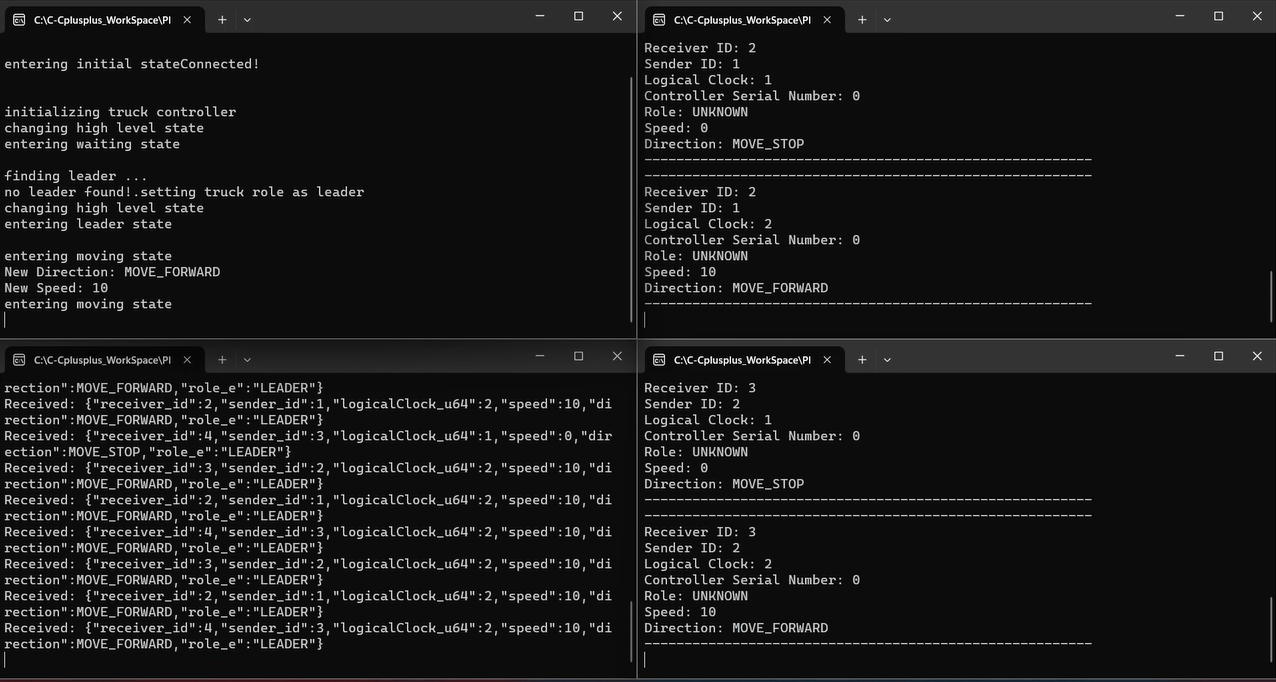
\includegraphics[width=0.5\textwidth]{images/SystemTest_Listen.png}
    \caption{Server listening test}
    \label{img:SystemTest_Listen}
\end{figure}

%%% SystemTest_Case
\begin{figure}[ht]
    \centering
    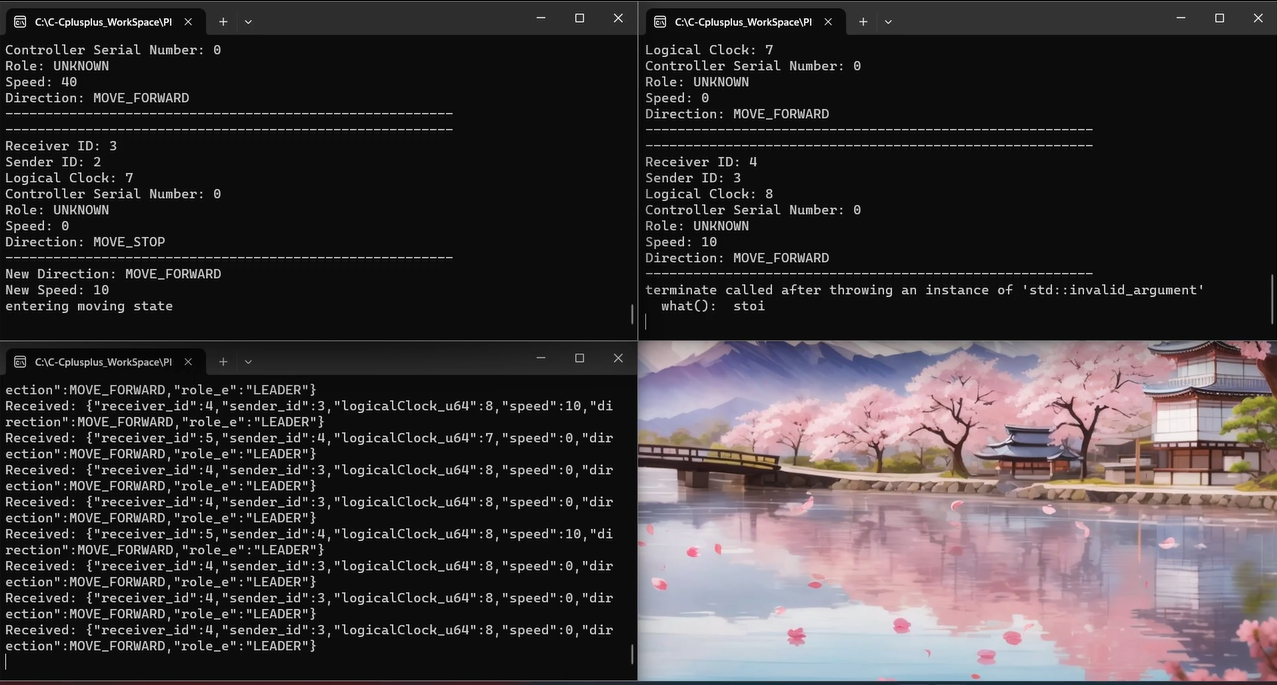
\includegraphics[width=0.5\textwidth]{images/SystemTest_Case.png}
    \caption{Leader lost test case}
    \label{img:SystemTest_Case}
\end{figure}

%%% code
\begin{lstlisting}[ language=c++, caption=Main Process of a truck using pthread, label = code:code_1]

// Create the threads that will be run in the system called: Truck

pthread_create(&t_communication, NULL, &CommsModule::run, &truck_communication);
pthread_create(&t_controller, NULL, &controller::run, &truck_controller);
pthread_create(&t_interface, NULL, &controller::key_board_run, &truck_controller);

// Run the threads so the actual simulation can be run through the thread id called:
// - t_controller
// - t_interface
// - t_communications

pthread_join(t_controller, NULL);
pthread_join(t_interface, NULL);
pthread_join(t_communication, NULL);

\end{lstlisting}

